% chktex-file 1
\documentclass{article}
% chktex-file 34
% chktex-file 18
% chktex-file 1
\usepackage{amsfonts}
\usepackage[T1]{fontenc}
\usepackage{amsmath}
\usepackage{amssymb}
\usepackage{mathrsfs}
\usepackage{extarrows}
\usepackage{hyperref}
\usepackage[utf8]{inputenc}
\usepackage{graphicx}
\usepackage{mathtools}
\usepackage[a4paper, total={6in, 8in}]{geometry}
\usepackage[table]{xcolor}
\usepackage{tikz}
\usepackage{cancel}
\usepackage{steinmetz}
\usepackage{diagbox}
\usepackage{siunitx}
\usepackage{eurosym}
\usepackage{pgfplots}
\pgfplotsset{width=10cm,compat=1.9}
\usetikzlibrary{shapes,arrows}
\usepackage{listings}
\usepackage{color}
%definizione colori per blocchi di codice
\definecolor{lightgray}{rgb}{.95,.95,.95}
\definecolor{darkgray}{rgb}{.4,.4,.4}
\definecolor{purple}{rgb}{0.65, 0.12, 0.82}
\definecolor{ocherCode}{rgb}{1, 0.5, 0}
\definecolor{blueCode}{rgb}{0, 0, 0.93}
\definecolor{greenCode}{rgb}{0, 0.6, 0}

%formattazione per i blocchi di codice
\lstset{
  %Special characters
  literate={á}{{\'a}}1 {é}{{\'e}}1 {í}{{\'\i}}1 {ó}{{\'o}}1 {ú}{{\'u}}1 {Á}{{\'A}}1 {É}{{\'E}}1 {Í}{{\'I}}1 {Ó}{{\'O}}1 {Ú}{{\'U}}1 {à}{{\`a}}1 {è}{{\`e}}1 {ì}{{\`\i}}1 {ò}{{\`o}}1 {ù}{{\`u}}1 {À}{{\`A}}1 {È}{{\`E}}1 {Ì}{{\`I}}1 {Ò}{{\`O}}1 {Ù}{{\`U}}1 {ä}{{\"a}}1 {ë}{{\"e}}1 {ï}{{\"\i}}1 {ö}{{\"o}}1 {ü}{{\"u}}1 {Ä}{{\"A}}1 {Ë}{{\"E}}1 {Ï}{{\"I}}1 {Ö}{{\"O}}1 {Ü}{{\"U}}1 {â}{{\^a}}1 {ê}{{\^e}}1 {î}{{\^\i}}1 {ô}{{\^o}}1 {û}{{\^u}}1 {Â}{{\^A}}1 {Ê}{{\^E}}1 {Î}{{\^I}}1 {Ô}{{\^O}}1 {Û}{{\^U}}1 {ã}{{\~a}}1 {ẽ}{{\~e}}1 {ĩ}{{\~\i}}1 {õ}{{\~o}}1 {ũ}{{\~u}}1 {Ã}{{\~A}}1 {Ẽ}{{\~E}}1 {Ĩ}{{\~I}}1 {Õ}{{\~O}}1 {Ũ}{{\~U}}1 {œ}{{\oe}}1 {Œ}{{\OE}}1 {æ}{{\ae}}1 {Æ}{{\AE}}1 {ß}{{\ss}}1 {ű}{{\H{u}}}1 {Ű}{{\H{U}}}1 {ő}{{\H{o}}}1 {Ő}{{\H{O}}}1 {ç}{{\c c}}1 {Ç}{{\c C}}1 {ø}{{\o}}1 {Ø}{{\O}}1 {å}{{\r a}}1 {Å}{{\r A}}1 {€}{{\euro}}1 {£}{{\pounds}}1 {«}{{\guillemotleft}}1 {»}{{\guillemotright}}1 {ñ}{{\~n}}1 {Ñ}{{\~N}}1 {¿}{{?`}}1 {¡}{{!`}}1 {'"'}{\textquotesingle "\textquotesingle}3,
  %Basic design
  backgroundcolor=\color{lightgray},
  frame=l,
  % Line numbers
  xleftmargin={0.75cm},
  numbers=left,
  numberstyle=\footnotesize,
  numbersep=9pt,
  stepnumber=1,
  firstnumber=1,
  numberfirstline=true,
  % Code design
  identifierstyle=\color{black},
  keywordstyle=\color{blue}\bfseries,
  ndkeywordstyle=\color{ocherCode}\bfseries,
  stringstyle=\color{greenCode}\ttfamily,
  commentstyle=\color{darkgray}\ttfamily,
  %Code
  columns=[c]fixed,
  extendedchars=true,
  upquote=true,
  breaklines=true,
  showstringspaces=false,
  showspaces=false,
  tabsize=2,
  breaklines=true,
  showtabs=false,
  captionpos=b
}
%lingue supportate:
%ABAP
%ACSL
%Ada
%Algol
%Ant
%Assembler
%Awk
%bash
%Basic
%C#5
%C++
%C
%Caml
%Clean
%Cobol
%Comal
%csh
%Delphi
%Eiffel
%Elan
%erlang
%Euphoria
%Fortran
%GCL
%Go (golang)
%Gnuplot
%Haskell
%HTML
%IDL
%inform
%Java
%JVMIS
%ksh
%Lisp
%Logo
%Lua
%make
%Mathematica
%Matlab
%Mercury
%MetaPost
%Miranda
%Mizar
%ML
%Modelica
%Modula-2
%MuPAD
%NASTRAN
%Oberon-2
%Objective C
%OCL
%Octave
%Oz
%Pascal
%Perl
%PHP
%PL/I
%Plasm
%POV
%Prolog
%Promela
%Python
%R
%Reduce
%Rexx
%RSL
%Ruby
%S4
%SAS
%Scilab
%sh
%SHELXL
%Simula
%SQL
%tcl4
%TeX
%VBScript
%Verilog
%VHDL
%VRML
%XML
%XSLT

\newcommand{\acapo}{\\\hspace*{1cm}\\}
\newcommand{\Eaccentata}{$\grave{\text{E}}$ }
\newcommand{\vopen}{``}
\newcommand{\apexopen}{`}
\newcommand{\vclose}{''}
\newcommand{\vclosespace}{'' }
\newcommand{\indenta}{\hspace*{1cm}}
\newcommand{\define}{\underline{Def:} }

\setlength{\parindent}{0cm}

\hfuzz=100pt

\author{Flavio Colacicchi}

\title{Alcune idee sui sistemi software e la loro architettura\\\normalsize Analisi e progettazione del software}
\date{13/03/2025}
\begin{document}
\maketitle
La scelta dell'architettura è una scelta scruciale da fare all'inizio dello sviluppo e che sarà difficile da cambiare in seguito, un'architettura comunq è quella a strati che interagiscono al seguente modo: gli strati alti possono fare chiamate a quelli più bassi ma non è vero il contrario. Una possibile scelta, minimale ma comune è la seguente
\begin{itemize}
    \item Presentazione\\
        UI e ha lo scopo di capire cosa vuole fare l'utente per poi fare una chiamata allo strato sottostante
    \item Lgica applicativa\\
        Delega la richiesta alla base di dati da cui otterrà dei dati che elabora e restituisce allo strato superiore per la presentazione all'utente    
    \item Accesso alla base di dati e altri servizi tecnici
\end{itemize}
\begin{center}
    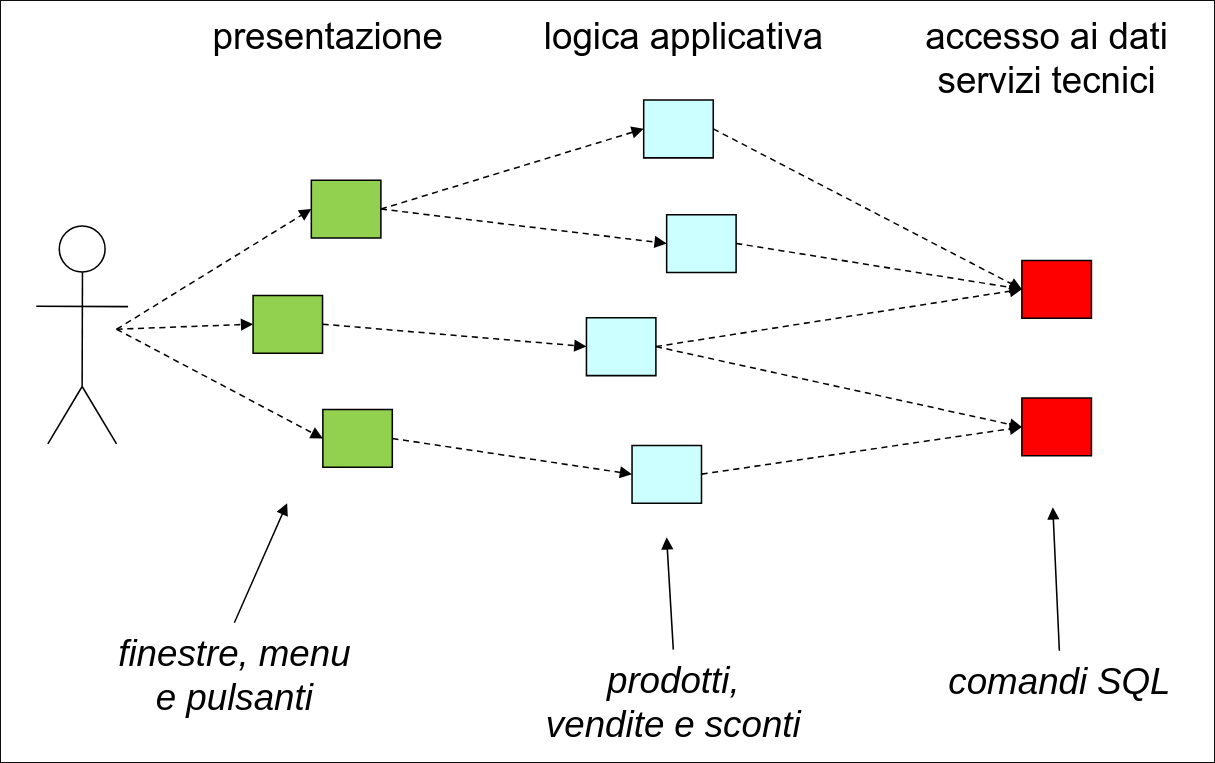
\includegraphics[width=10cm]{images/architettura a strati.png}
\end{center}
La scelta del modo in cui è organizzato lo strato della logica operativa influisce pesantemente sul metodo per l'analisi del softawre, ci sono diversti approcci:
\begin{itemize}
    \item Approccio \vopen tradizionale\vclose
        \begin{itemize}
            \item I dati sono gesitit da una base di dati
            \item Le operazioni sono transazioni sulla base di dati, ciascun oggetto/classe della logica applicativa corrisponde a una procedura/transazione che l'utente può richiedere al sistema\\
            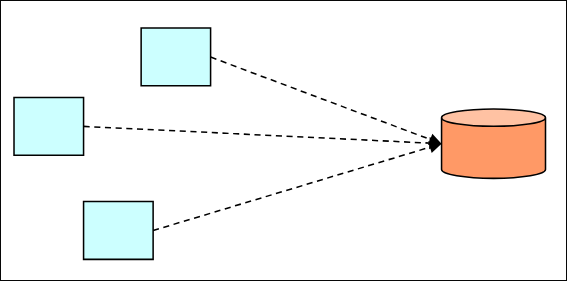
\includegraphics[width=6cm]{images/approccio tradizionale.png}
        \end{itemize}
    \item Approccio \vopen procedurale\vclose
        \begin{itemize}
            \item I dati sono gestiti in memoria principale
            \item Alcuni oggetti sono usati per rappresentarre dati/informazioni
            \item Altri oggetti (separati) definiscono le operazioni che possono essere applicate alle informazioni, a maggior parte di questi oggetti di dominio incapsulano sia dati che operazioni\\
            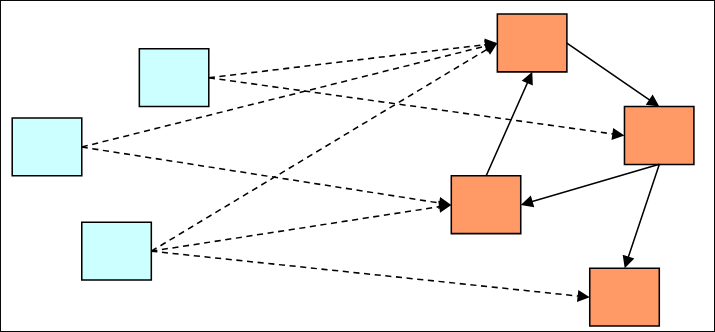
\includegraphics[width=6cm]{images/approccio procedurale.png}
        \end{itemize}
    \item Domani model
        \begin{itemize}
            \item lo strato della logica applicativa è realizzato a oggetti che si ripartiscono le responsabilità del sistema
            \item lo strato della logica applicativa viene anche chiamato strato
            di dominio\\
            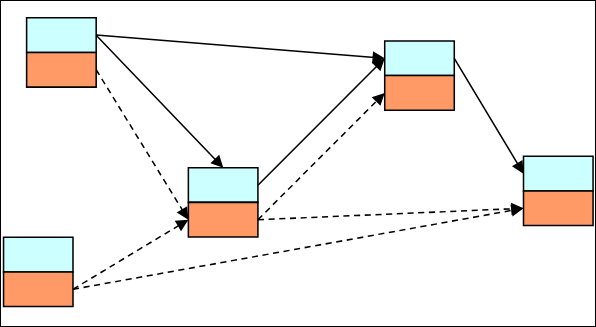
\includegraphics[width=6cm]{images/strato di dominio.png}
        \end{itemize}
\end{itemize}
\Large Per quanto riguarda l'organizzazione della logica applicativa, questo corso fa riferimento alla strategia Domain Model\normalsize\acapo
In generale un'applicazione software offre ai suoi utilizzatori un certo numero di funzionalità che sono relative alla gestione di alcuni tipi di informazioni (dati).\newpage
\Eaccentata utile distinguere tra due tipologie principali:
\begin{itemize}
    \item Applicazioni stand-alone (monopoly)\\
        Applicazioni mono-utente i cui dati non sono condivisi con utenti diversi della stessa applicazione
        \begin{center}
            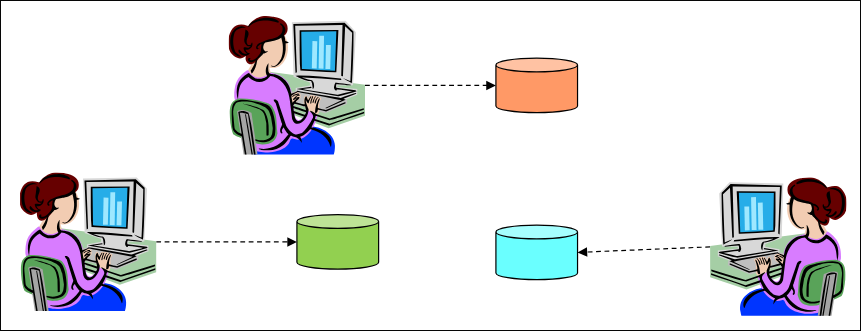
\includegraphics[width=6cm]{images/applicazioni standalone.png}
        \end{center}
    \item Applicazioni client-server\\
        Applicazioni che possono essere accedute in modo concorrente da più utenti tramite acesso in rete o sul web\\
        Queste applicazioni gestiscono in genere anche i dati che devono essere condivisi dall'utente
        \begin{center}
            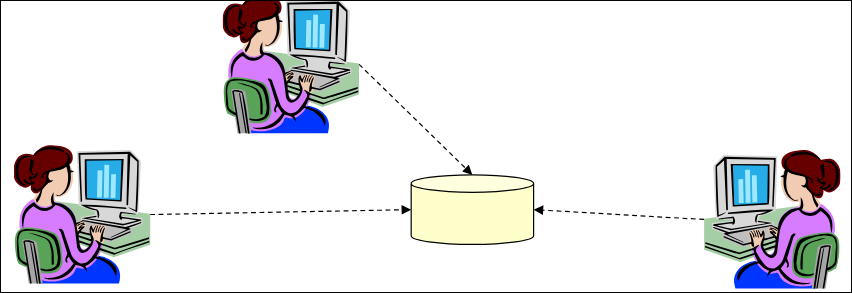
\includegraphics[width=6cm]{images/applicazioni client server.png}
        \end{center}
\end{itemize}
Per la progettazione
\begin{itemize}
    \item Il caso di un'applicazione stand-alone è relativamente semplice\\
        \Eaccentata infatti sufficiente pensare a una singola istanza/esecuzione dellapplicazione, dal punto di vista di un singolo utente
    \item Il caso di un'applicazione client server è molto più complesso\\
        Da una parte, l'applicazione deve gestire alcuni dati condivisi tra tutti i suoi utenti/client\\
        Inoltre, per ciascun utente/client, l'applicazione deve gestire alcuni dati specifici per la conversazione/sessione con quel particolare client
\end{itemize}
Dunque un'applicazione client/server per quanto riguarda lo stato delle sessioni in questo corso ipotiziamo di utilizzare una tecnologia che consenta di ragionare (e scrivere programmi) in termini di singola conversazione/sessione. Una soluzione comune è l'introduzione di un ulteriore strato (\vopen application\vclose) tra quello di presentazione e quello della logica
\begin{center}
    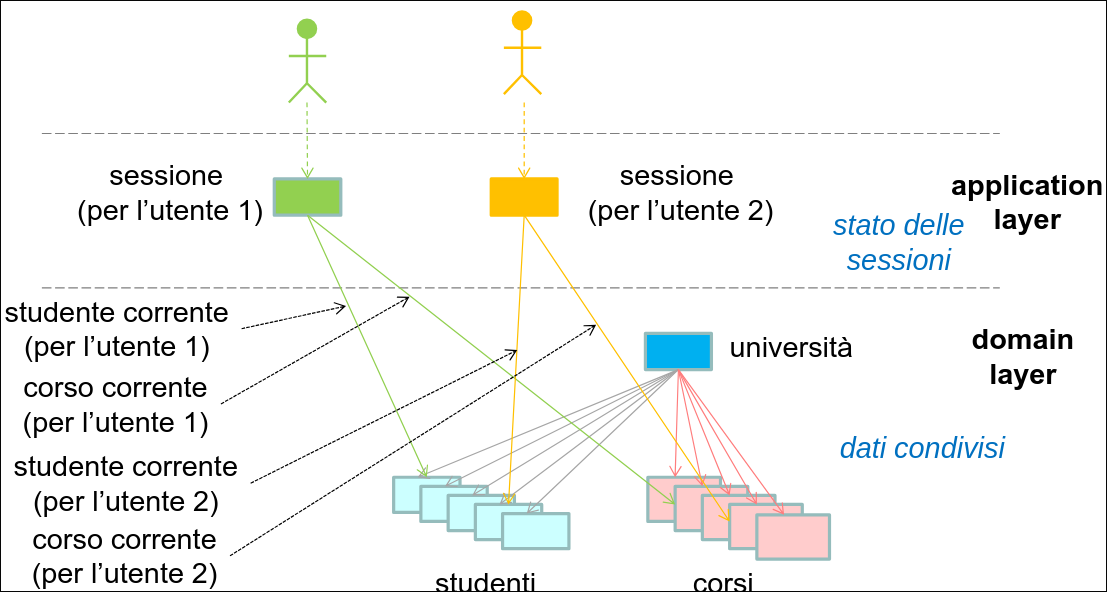
\includegraphics[width=8cm]{images/application layer.png}
\end{center}
\end{document}